\documentclass[10pt]{beamer}
\usetheme[
%%% options passed to the outer theme
%    hidetitle,           % hide the (short) title in the sidebar
%    hideauthor,          % hide the (short) author in the sidebar
%    hideinstitute,       % hide the (short) institute in the bottom of the sidebar
%    shownavsym,          % show the navigation symbols
%    width=2cm,           % width of the sidebar (default is 2 cm)
%    hideothersubsections,% hide all subsections but the subsections in the current section
%    hideallsubsections,  % hide all subsections
%    left                % right of left position of sidebar (default is right)
  ]{Aalborg}
  
% If you want to change the colors of the various elements in the theme, edit and uncomment the following lines
% Change the bar and sidebar colors:
%\setbeamercolor{Aalborg}{fg=red!20,bg=red}
%\setbeamercolor{sidebar}{bg=red!20}
% Change the color of the structural elements:
%\setbeamercolor{structure}{fg=red}
% Change the frame title text color:
%\setbeamercolor{frametitle}{fg=blue}
% Change the normal text color background:
%\setbeamercolor{normal text}{bg=gray!10}
% ... and you can of course change a lot more - see the beamer user manual.

\usepackage[utf8]{inputenc}
\usepackage[spanish]{babel}
\usepackage[T1]{fontenc}
% Or whatever. Note that the encoding and the font should match. If T1
% does not look nice, try deleting the line with the fontenc.

\usepackage[table,xcdraw]{xcolor}
\usepackage{helvet}
\usepackage{tikz}
\usetikzlibrary{shapes,arrows,positioning}

\usepackage{minted}


\usepackage{listings}
\usepackage{color}
\definecolor{codegreen}{rgb}{0,0.6,0}
\definecolor{codegray}{rgb}{0.5,0.5,0.5}
\definecolor{codepurple}{rgb}{0.58,0,0.82}
\definecolor{backcolour}{rgb}{0.95,0.95,0.92}
 
\lstdefinestyle{mystyle}{
    backgroundcolor=\color{backcolour},   
    commentstyle=\color{codegreen},
    keywordstyle=\color{magenta},
    numberstyle=\tiny\color{codegray},
    stringstyle=\color{codepurple},
    basicstyle=\footnotesize,
    breakatwhitespace=false,         
    breaklines=true,                 
    captionpos=b,                    
    keepspaces=true,                 
    numbers=left,                    
    numbersep=5pt,                  
    showspaces=false,                
    showstringspaces=false,
    showtabs=false,                  
    tabsize=2
}
 
\lstset{style=mystyle}


% colored hyperlinks
\newcommand{\chref}[2]{%
  \href{#1}{{\usebeamercolor[bg]{Aalborg}#2}}%
}

\title[Sensores y Actuadores]% optional, use only with long paper titles
{Sensores y Actuadores}

\subtitle{Git y Github para poetas, parte 4}  % could also be a conference name

\date{\today}

\author[Víctor Medrano Zarazúa] % optional, use only with lots of authors
{
  Víctor Medrano Zarazúa\\
  \href{mailto:victor.medranozr@uanl.edu.mx}{{\tt victor.medranozr@uanl.edu.mx}}
}
% - Give the names in the same order as they appear in the paper.
% - Use the \inst{?} command only if the authors have different
%   affiliation. See the beamer manual for an example

\institute[
%  {\includegraphics[scale=0.2]{aau_segl}}\\ %insert a company, department or university logo
  %Dept.\ of Electronic Systems\\
  Universidad Autónoma de Nuevo León\\
  Facultad de Ingeniería Mecánica y Eléctrica
] % optional - is placed in the bottom of the sidebar on every slide
{% is placed on the bottom of the title page
  %Department of Electronic Systems\\
  Universidad Autónoma de Nuevo León\\
  Facultad de Ingeniería Mecánica y Eléctrica
  
  %there must be an empty line above this line - otherwise some unwanted space is added between the university and the country (I do not know why;( )
}

% specify the logo in the top right/left of the slide
\pgfdeclareimage[height=1cm]{mainlogo}{AAUgraphics/FIME} % placed in the upper left/right corner
\logo{\pgfuseimage{mainlogo}}

% specify a logo on the titlepage (you can specify additional logos an include them in 
% institute command below
\pgfdeclareimage[height=1.5cm]{titlepagelogo}{AAUgraphics/UANL} % placed on the title page
%\pgfdeclareimage[height=1.5cm]{titlepagelogo2}{AAUgraphics/aau_logo_new} % placed on the title page
\titlegraphic{% is placed on the bottom of the title page
  \pgfuseimage{titlepagelogo}
%  \hspace{1cm}\pgfuseimage{titlepagelogo2}
}

%\definecolor{UniBlue}{RGB}{255,255,255}

\tikzset{
block/.style={
  draw, 
  fill=blue!20, 
  rectangle, 
  minimum height=3em, 
  minimum width=6em
  },
 gain/.style={
    draw,
    fill=blue!20, 
    isosceles triangle,
    minimum height = 3em,
    isosceles triangle apex angle=60
    },
sum/.style={
  draw, 
  fill=blue!20, 
  circle, 
  },
input/.style={coordinate},
output/.style={coordinate},
pinstyle/.style={
  pin edge={to-,thin,black}
  }
}  

\begin{document}
% the titlepage


%\setbeamercolor{title}{fg=UniBlue}
%\setbeamercolor{normal text}{fg=UniBlue}
%\setbeamercolor{Aalborg}{fg=black,bg=black}


{\aauwavesbg
\begin{frame}[plain,noframenumbering] % the plain option removes the sidebar and header from the title page
  \titlepage
\end{frame}}
%%%%%%%%%%%%%%%%

% TOC
\begin{frame}{Contenido}{}
\tableofcontents
\end{frame}
%%%%%%%%%%%%%%%%
\section{Repaso}
\begin{frame}{Repaso}{}
\begin{block}{Recapítulemos...}
\begin{itemize}
    \item ¿Qué es un issue?
    \item ¿Para qué sirve un issue?
    \item ¿De qué plataforma forma parte el concepto de issue?
    \item ¿Qué es Markdown?
\end{itemize}
\end{block}

%\begin{figure}[h!]
%\centering
%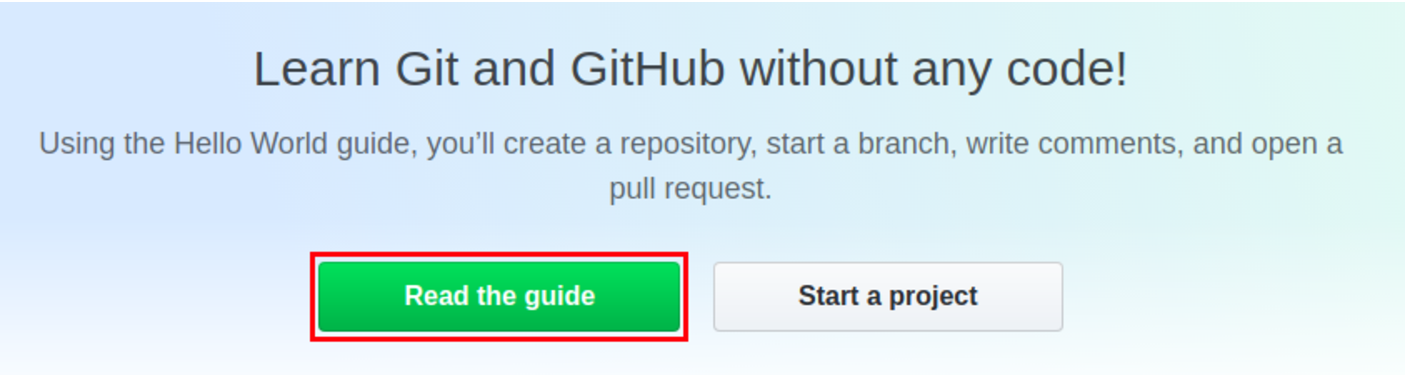
\includegraphics [scale=0.32]{github}
%\caption{Bobina Tesla}
%\label{fig:tesla}
%\end{figure}

\end{frame}

\section{Introducción}

\begin{frame}{Introducción}{}
\begin{block}{Git y la terminal}
\medskip
\begin{columns}[c]
\column{2in}
\begin{itemize}
    \item Veremos cómo mantener un control de versiones con archivos almacenados localmente en nuestra computadora. 
    \item Usaremos Git de forma offline y sin necesidad de acceder al sitio de Github.
    \item Veremos los comandos principales a ejecutar en una terminal y haremos uso de comandos de Git para administrar repositorios.
\end{itemize}

\column{1.5in}
\framebox{
\includegraphics[width=1.5in]{terminal.png}}
\end{columns}
\end{block}
\end{frame}

\section{Terminal}

\begin{frame}{Terminal}{Abriendo la terminal}
\begin{block}{Según tu sistema operativo...}

%\begin{columns}[c]
%\column{2.3in}
%\vspace{-0.2in}
\begin{itemize}
        \item Si eres usuario de Mac o Linux, puedes hacer uso de la terminal que ya está incluida en el mismo sistema operativo.\\
        
        \item Si eres usuario de Windows se recomienda bajar el Git bash haciendo clic en el \href{https://git-scm.com/downloads}{\textcolor{blue}{enlace}}, ya que usaremos comandos de Unix/Linux.
\end{itemize}

%\column{1.3in}
%\framebox{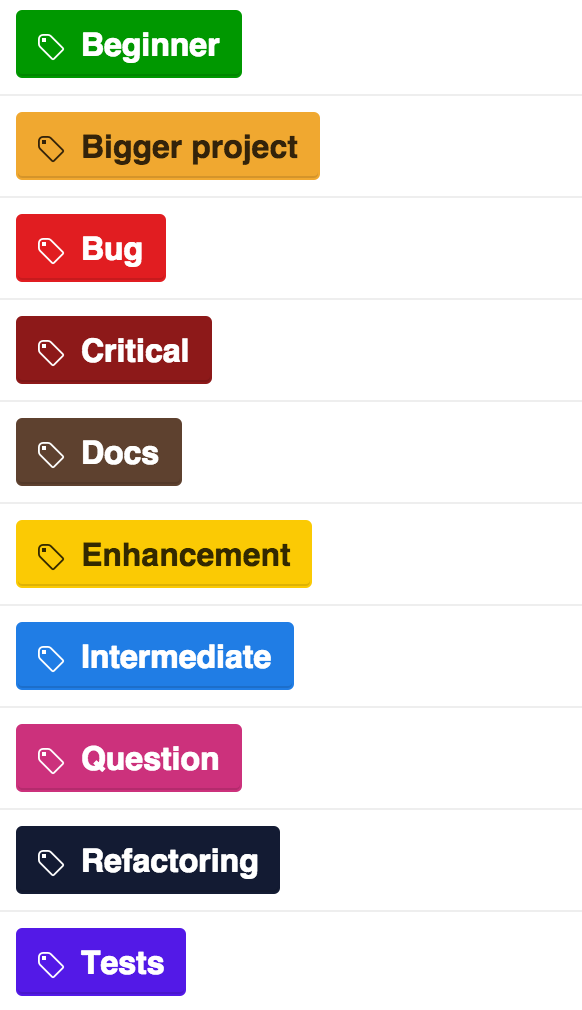
\includegraphics[width=1.3in]{issueslabels.png}}
%\end{columns}
    
\end{block}

\end{frame}

\begin{frame}{Terminal}{Bash terminal}
\begin{block}{¿Qué es el bash/terminal?}

%\begin{columns}[c]
%\column{2.3in}
%\vspace{-0.2in}
Es un intérprete de comandos que ejecuta tareas específicas dentro del sistema operativo.

\begin{figure}[h!]
\centering
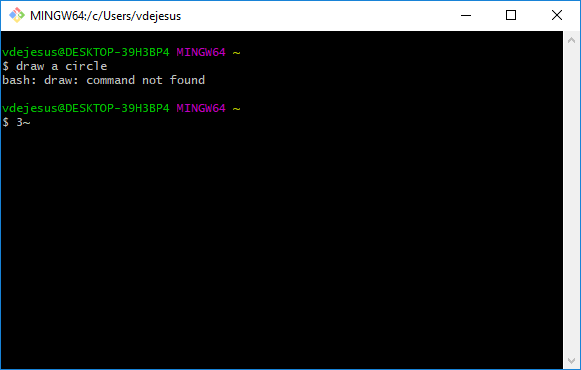
\includegraphics [scale=0.45]{bash}
%\caption{Sección de Issues}
\label{fig:bash}
\end{figure}

%\column{1.3in}
%\framebox{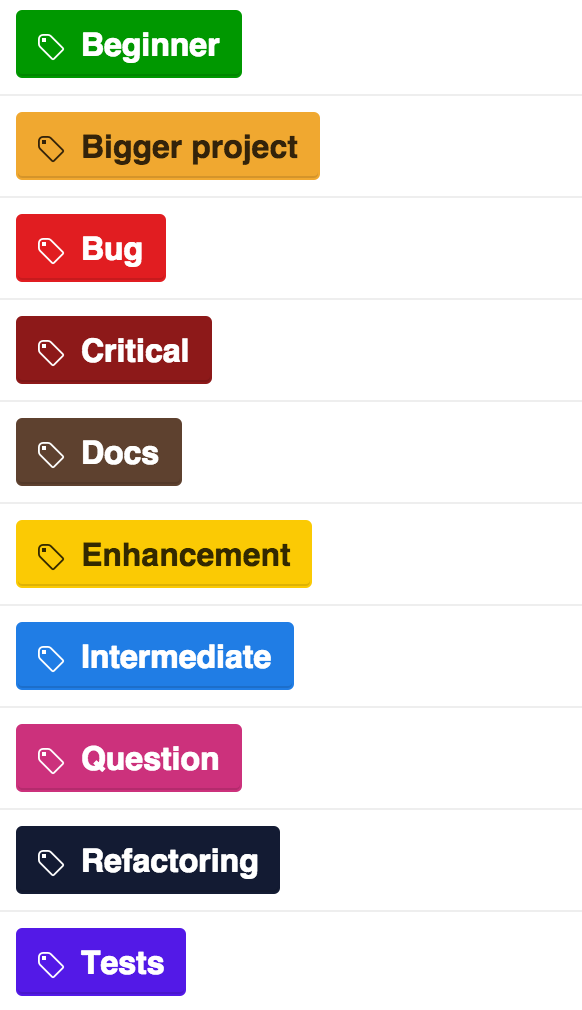
\includegraphics[width=1.3in]{issueslabels.png}}
%\end{columns}
    
\end{block}

\end{frame}

\begin{frame}{Terminal}{Comandos principales}

\begin{block}{}

%\begin{columns}[c]
\begin{itemize}
        \item cd (cambia de directorio)
        \item pwd (print working directory, muestra el directorio actual)
        \item ls (hace una lista de los archivos dentro del directorio actual)
        \item clear (limpia la terminal)
        \item help (muestra ayuda para diferentes comandos)
\end{itemize}
    
\end{block}

\end{frame}

\begin{frame}{Terminal}{Cosas que debes saber}

\begin{block}{}

%\begin{columns}[c]
\begin{itemize}
        \item Para regresar un directorio hacia arriba hacemos uso del comando \textcolor{blue}{cd ..}
        \item La tecla \textit{TAB} sirve para evitar teclear el nombre completo de un archivo o directorio. Nos ahorra tiempo al navegar por el sistema de archivos.
        \item Las teclas ↑ y ↓ nos permiten navegar a través de los comandos previos que hemos introducido en la terminal.
        \item Podemos arrastrar directorios hacia la terminal para obtener de forma automática la ruta que poseen en el sistema de archivos.
        \item Los comandos de Unix/Linux frecuentemente son modificados con argumentos (e.g: \textcolor{blue}{ls} \textcolor{red}{-all})
\end{itemize}
    
\end{block}

\end{frame}

\section{Git}

\begin{frame}{Git}{Introducción}

\begin{block}{Git ready...}

%\begin{columns}[c]
Asegurando que la instalación de Git se haya hecho correctamente, teclearemos el comando \textcolor{blue}{git}.

\begin{figure}[h!]
\centering
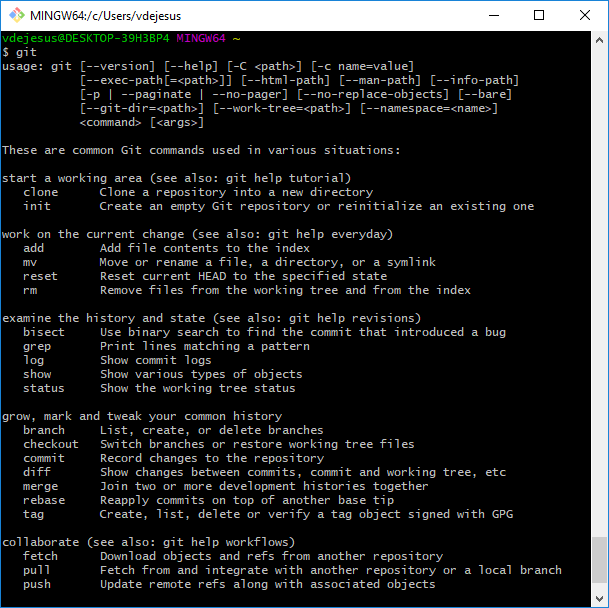
\includegraphics [scale=0.35]{gitback}
%\caption{Sección de Issues}
\label{fig:git}
\end{figure}

\end{block}

\end{frame}

\begin{frame}{Terminal}{Introducción}

\begin{block}{Not a git repository...}

%\begin{columns}[c]
Intentando hacer un commit. Pero el esfuerzo es infructuoso :(


\begin{figure}[h!]
\centering
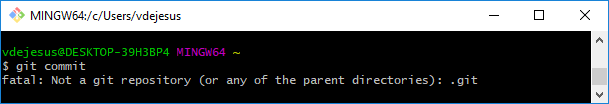
\includegraphics [scale=0.55]{notgit}
%\caption{Sección de Issues}
\label{fig:notgit}
\end{figure}

\end{block}

\end{frame}

\begin{frame}{Terminal}{Introducción}

\begin{block}{Repositorios locales}

%\begin{columns}[c]
Anteriormente estuvimos trabajando con repositorios alojados en el sitio web de Github. Ahora veremos como crear y administrar estos repositorios de forma local en nuestra PC.


\begin{figure}[h!]
\centering
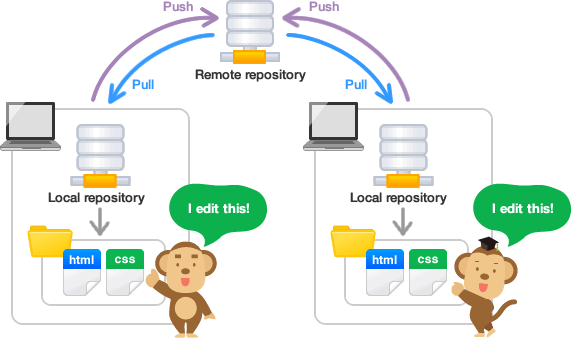
\includegraphics [scale=0.35]{localremote}
%\caption{Sección de Issues}
\label{fig:localremote}
\end{figure}

\end{block}

\end{frame}

\begin{frame}{Git}{Clonando repos y haciendo push}

\begin{block}{It's a new dawn, it's a new day, it's a new life...}

%\begin{columns}[c]
\begin{itemize}
        \item La forma más sencilla de empezar es hacer un repositorio en Github y después ``descargarlo'' en nuestra computadora. A este proceso de ``descargar'' un repositorio lo llamaremos formalmente como \textcolor{blue}{clone} (primera vez) o \textcolor{blue}{pull} (actualizar repositorio).
        \item Se le llama clonar a la acción de tomar un repositorio remoto y almacenarlo como una copia en un repositorio local.
        \item Se pueden hacer cambios en el repositorio local y hacer \textcolor{blue}{push} en el repositorio remoto para actualizarlo. O viceversa, puede haber cambios en el repositorio remoto y haremos \textcolor{blue}{pull} para actualizar el repositorio local.
\end{itemize}

\end{block}

\end{frame}

\begin{frame}{Git}{Clonando repos y haciendo push}

\begin{block}{Clonando repositorio}

%\begin{columns}[c]
Se crea un repositorio en Github y se copia el enlace del mismo como muestra la imagen de abajo.

\begin{figure}[h!]
\centering
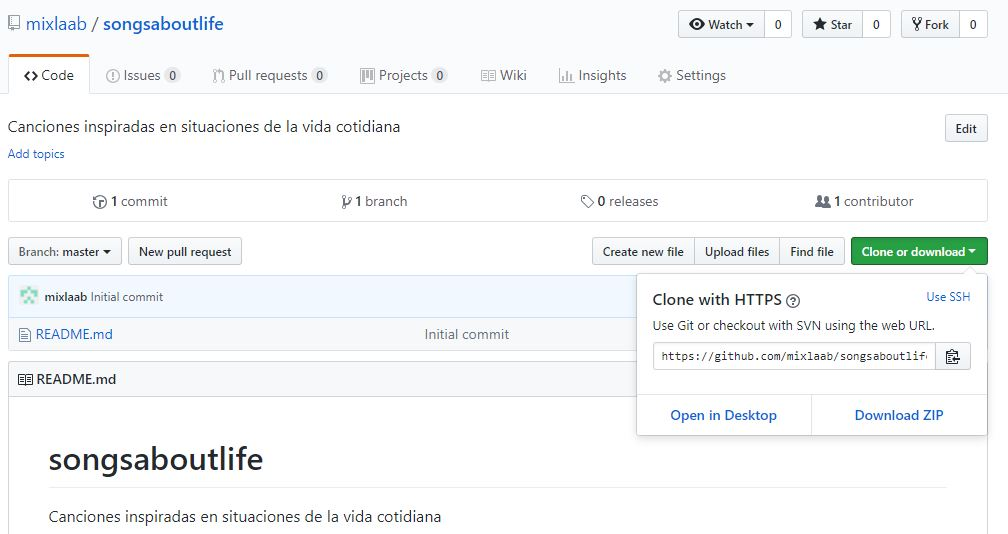
\includegraphics [scale=0.35]{songsaboutlife}
%\caption{Sección de Issues}
\label{fig:songs}
\end{figure}

\end{block}

\end{frame}

\begin{frame}{Git}{Clonando repos y haciendo push}

\begin{block}{Clonando repositorio}

%\begin{columns}[c]
Hacemos uso del comando git clone.

\begin{figure}[h!]
\centering
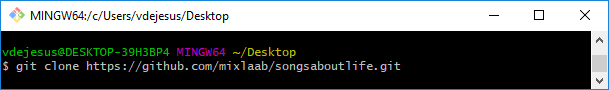
\includegraphics [scale=0.5]{gitclone}
%\caption{Sección de Issues}
\label{fig:gitclone}
\end{figure}

\end{block}

\end{frame}

\begin{frame}{Git}{Clonando repos y haciendo push}

\begin{block}{Clonando repositorio}

%\begin{columns}[c]
%Hacemos uso del comando git clone.

\begin{figure}[h!]
\centering
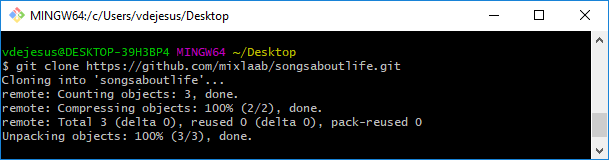
\includegraphics [scale=0.5]{gitclone2}
%\caption{Sección de Issues}
\label{fig:gitclone2}
\end{figure}

\end{block}

\end{frame}

\begin{frame}{Git}{Clonando repos y haciendo push}

\begin{block}{Clonando repositorio}
Usando el comando \textcolor{blue}{ls}.
%\begin{columns}[c]
%Hacemos uso del comando git clone.

\begin{figure}[h!]
\centering
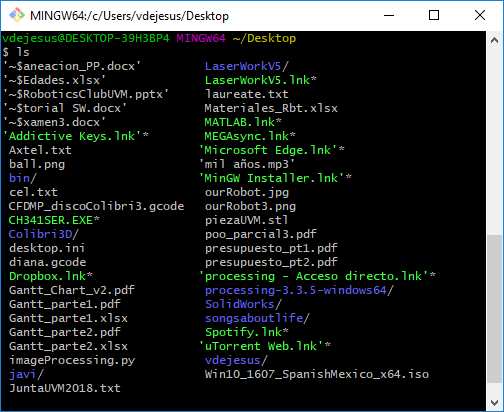
\includegraphics [scale=0.5]{gitclone3}
%\caption{Sección de Issues}
\label{fig:gitclone3}
\end{figure}

\end{block}

\end{frame}

\begin{frame}{Git}{Clonando repos y haciendo push}

\begin{block}{Status del repositorio}
Usando el comando git status. Debemos estar dentro del directorio del repositorio para que el comando funcione.
%\begin{columns}[c]
%Hacemos uso del comando git clone.

\begin{figure}[h!]
\centering
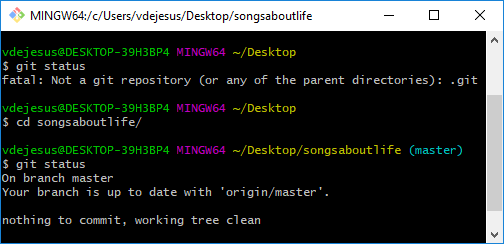
\includegraphics [scale=0.5]{gitstatus}
%\caption{Sección de Issues}
\label{fig:gitstatus}
\end{figure}

\end{block}

\end{frame}

\begin{frame}{Git}{Clonando repos y haciendo push}

\begin{block}{Modificando archivos de forma local}
Necesitaremos un editor de código. En lo personal recomiendo alguno de los siguientes:

\begin{itemize}
    \item Visual Studio Code
    \item Brackets
    \item Sublime Text
\end{itemize}

\begin{figure}[h!]
\centering
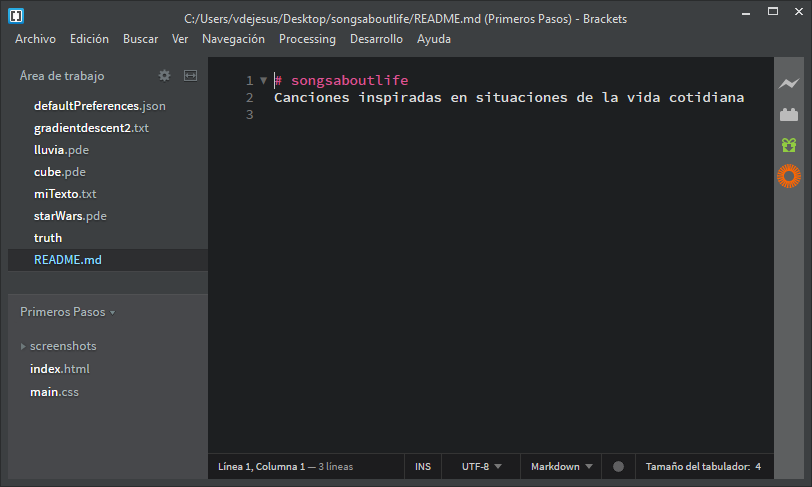
\includegraphics [scale=0.3]{brackets}
%\caption{Sección de Issues}
\label{fig:brackets}
\end{figure}

%\begin{columns}[c]
%Hacemos uso del comando git clone.

\end{block}

\end{frame}

\begin{frame}{Git}{Clonando repos y haciendo push}

\begin{block}{Modificando archivos de forma local}

Modificamos el archivo y lo guardamos.

\begin{figure}[h!]
\centering
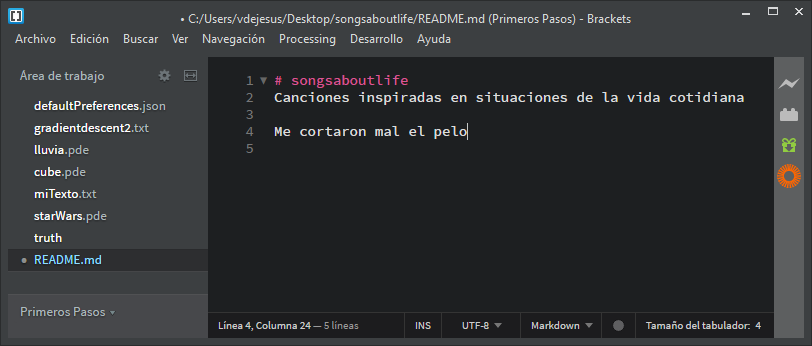
\includegraphics [scale=0.45]{filechange}
%\caption{Sección de Issues}
\label{fig:filechange}
\end{figure}
%\begin{columns}[c]
%Hacemos uso del comando git clone.

\end{block}

\end{frame}

\begin{frame}{Git}{Clonando repos y haciendo push}

\begin{block}{Modificando archivos de forma local}

Checamos el status del repositorio y veremos que hay una modificación en el archivo README.md

\begin{figure}[h!]
\centering
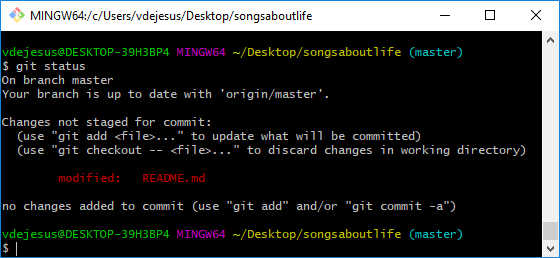
\includegraphics [scale=0.45]{gitstatus2}
%\caption{Sección de Issues}
\label{fig:gitstatus2}
\end{figure}
%\begin{columns}[c]
%Hacemos uso del comando git clone.

\end{block}

\end{frame}

\begin{frame}{Git}{Clonando repos y haciendo push}

\begin{block}{Haciendo push al repositorio remoto de Github}

Sin embargo aún no hay cambios en el repositorio remoto. Para lograr traspasar los cambios al repositorio de Github comenzaremos usando el comando \textcolor{blue}{git commit} \textcolor{red}{-a}. Es necesario haber accedido previamente los datos de nuestra cuenta, de lo contario sucederá lo siguiente...

\begin{figure}[h!]
\centering
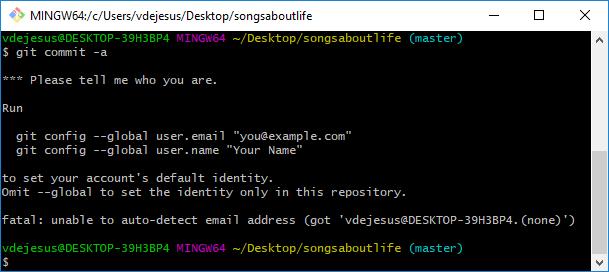
\includegraphics [scale=0.45]{gitcommit}
%\caption{Sección de Issues}
\label{fig:gitcommit}
\end{figure}
%\begin{columns}[c]
%Hacemos uso del comando git clone.

\end{block}

\end{frame}

\begin{frame}{Git}{Clonando repos y haciendo push}

\begin{block}{Haciendo push al repositorio remoto de Github}

Proporcionamos nuestro nombre de usuario en Github y la cuenta de correo asociada a la cuenta.

\begin{figure}[h!]
\centering
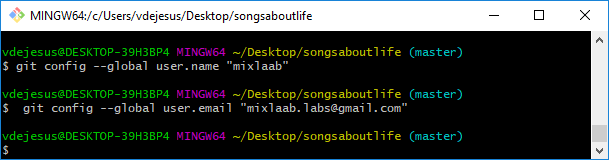
\includegraphics [scale=0.6]{gitlogin}
%\caption{Sección de Issues}
\label{fig:gitlogin}
\end{figure}
%\begin{columns}[c]
%Hacemos uso del comando git clone.

\end{block}

\end{frame}


\begin{frame}{Git}{Clonando repos y haciendo push}

\begin{block}{Haciendo push al repositorio remoto de Github}

Verificamos que los datos introducidos sean correctos con \textcolor{blue}{git config} \textcolor{red}{-{}-list.}

\begin{figure}[h!]
\centering
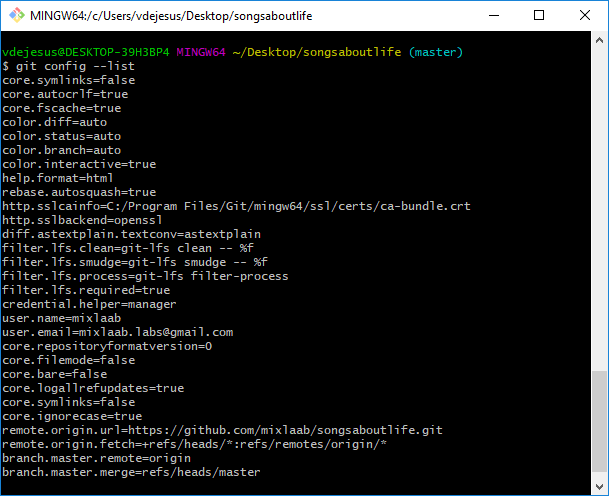
\includegraphics [scale=0.44]{configlist}
%\caption{Sección de Issues}
\label{fig:configlist}
\end{figure}
%\begin{columns}[c]
%Hacemos uso del comando git clone.

\end{block}

\end{frame}

\begin{frame}{Git}{Clonando repos y haciendo push}

\begin{block}{Haciendo push al repositorio remoto de Github}

Y ya podremos hacer commit. Además podremos agregar un título para ese commit utilizando el argumento \textcolor{red}{-m}.

\begin{figure}[h!]
\centering
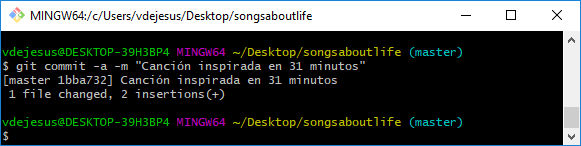
\includegraphics [scale=0.6]{gitcommit2}
%\caption{Sección de Issues}
\label{fig:gitcommit2}
\end{figure}
%\begin{columns}[c]
%Hacemos uso del comando git clone.

\end{block}

\end{frame}

\begin{frame}{Git}{Clonando repos y haciendo push}

\begin{block}{Haciendo push al repositorio remoto de Github}

Si vemos el status del repositorio aparecerá lo siguiente.

\begin{figure}[h!]
\centering
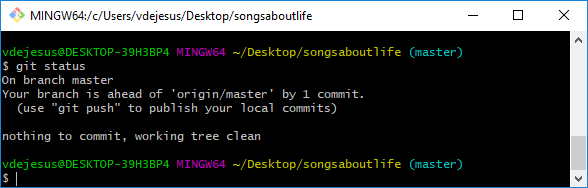
\includegraphics [scale=0.6]{gitstatus3}
%\caption{Sección de Issues}
\label{fig:gitstatus3}
\end{figure}
%\begin{columns}[c]
%Hacemos uso del comando git clone.

\end{block}

\end{frame}

\begin{frame}{Git}{Clonando repos y haciendo push}

\begin{block}{Haciendo push al repositorio remoto de Github}

Podemos ver un historial de los commits haciendo uso del comando \textcolor{blue}{git log}.

\begin{figure}[h!]
\centering
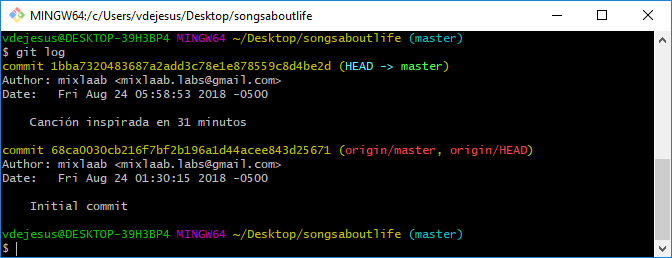
\includegraphics [scale=0.55]{gitlog}
%\caption{Sección de Issues}
\label{fig:gitlog}
\end{figure}
%\begin{columns}[c]
%Hacemos uso del comando git clone.

\end{block}

\end{frame}

\begin{frame}{Git}{Clonando repos y haciendo push}

\begin{block}{Haciendo push al repositorio remoto de Github}

También podemos ver una lista de los servidores remotos asociados al repositorio con el comando \textcolor{blue}{git remote} antes de hacer push.

\begin{figure}[h!]
\centering
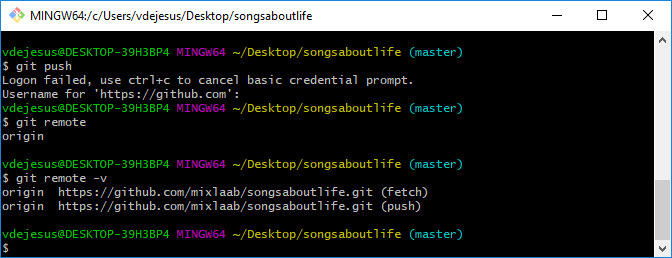
\includegraphics [scale=0.55]{gitremote}
%\caption{Sección de Issues}
\label{fig:gitlog}
\end{figure}
%\begin{columns}[c]
%Hacemos uso del comando git clone.

\end{block}

\end{frame}

\begin{frame}{Git}{Clonando repos y haciendo push}

\begin{block}{Haciendo push al repositorio remoto de Github}

Finalmente hago push al repositorio remoto (\textcolor{blue}{origin}) en la rama pertinente (en este caso, \textcolor{blue}{master}). Es necesario introducir usuario y contraseña del servidor remoto.
\medskip
\begin{columns}[c]
\column{2.5in}
\framebox{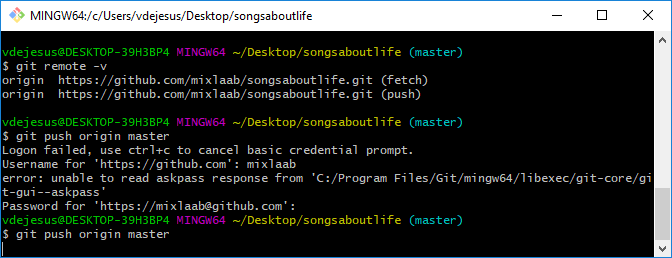
\includegraphics[width=2.5in]{gitpush.png}}
\column{1in}
\framebox{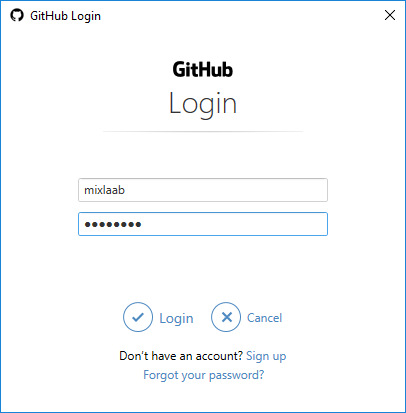
\includegraphics[width=1in]{gitpush2.png}}
\end{columns}


\end{block}

\end{frame}

\begin{frame}{Git}{Clonando repos y haciendo push}

\begin{block}{Haciendo push al repositorio remoto de Github}

Lo hicimos. Hemos actualizado el repositorio remoto.

\medskip

\begin{figure}[h!]
\centering
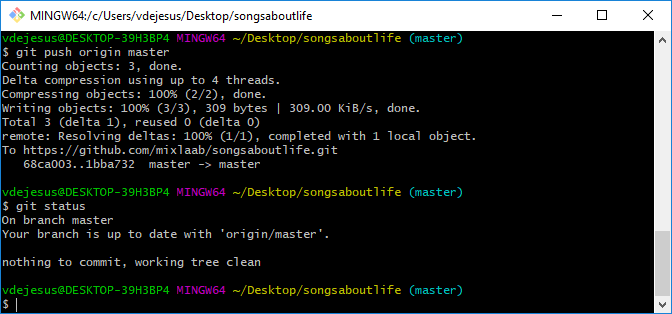
\includegraphics [scale=0.55]{eureka}
%\caption{Sección de Issues}
\label{fig:gitlog}
\end{figure}

\end{block}

\end{frame}

\begin{frame}{Git}{Clonando repos y haciendo push}

\begin{block}{Haciendo push al repositorio remoto de Github}

%Lo hicimos. Hemos actualizado el repositorio remoto.

\medskip

\begin{figure}[h!]
\centering
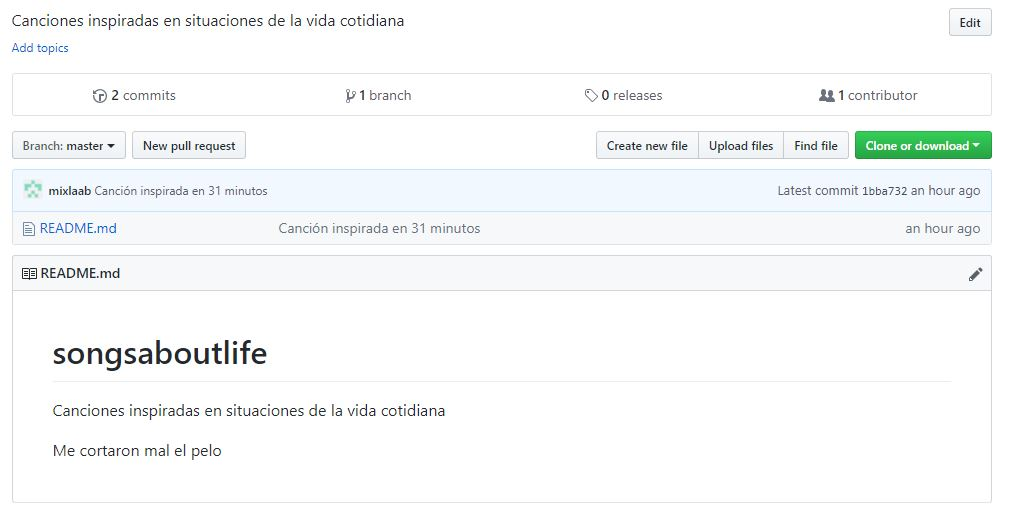
\includegraphics [scale=0.36]{eureka2}
%\caption{Sección de Issues}
\label{fig:gitlog}
\end{figure}

\end{block}

\end{frame}


\section{Tarea}
\begin{frame}{Tarea}{Usando la terminal para clonar, hacer commits y push}
\begin{block}{Tarea \#4 (Individual)}
\vspace{0.1in}
\begin{itemize}
    \item Crear un repositorio en el sitio de Github (debe contener archivo README.md). Recuerda poner una descripción a tu repositorio.
    \item Clonar el repositorio remoto en el repositorio local (tu PC).
    \item Modificar el archivo README.md localmente por medio de un editor de texto.
    \item Configurar nombre de usuario y correo antes de hacer commit.
    \item Hacer commit junto con un mensaje usando el argumento \textcolor{red}{-m}.
    \item Hacer push al repositorio remoto (recuerda que te pedirá nombre de usuario y contraseña de Github).
\end{itemize}

\end{block}
\end{frame}

\section{Información de contacto}
% contact information
\begin{frame}{Feedback}{Información de contacto}
En caso de comentarios, sugerencias, preguntas o errores en las diapositivas no dudes en contactarme.
  \begin{center}
    \insertauthor\\
    \chref{https://mixlaab.github.io}{https://mixlaab.github.io}\\
    WA: 8119022700\\
    %9220 Aalborg Ø
  \end{center}
\end{frame}
%%%%%%%%%%%%%%%%

{\aauwavesbg%
\begin{frame}[plain,noframenumbering]%
  \finalpage{Fin}
\end{frame}}
%%%%%%%%%%%%%%%%

\end{document}
